\documentclass{llncs}

\usepackage{graphicx}
%\usepackage{subfig}

\usepackage{caption, subcaption}

\captionsetup{compatibility=false}

\usepackage{url}
\usepackage{courier}
\usepackage{listings}

%!TEX root = ./paper1.tex

\lstset{
  float=tb,
	captionpos=b,
	breaklines=true,
	xleftmargin=20pt,
	basicstyle=\ttfamily\scriptsize,
	numberstyle=\tiny,
	flexiblecolumns=true,
	numbers=left,
	nolol=false,
	tabsize=2
}

\lstdefinelanguage{OCL}{
morekeywords={import,if,then,else,endif,self,and,true,false,def,includes,OclElement,package,let,in},
sensitive=true,
morecomment=[l]{--},
morestring=[b]",
morestring=[b]',
showstringspaces=false
}

\lstdefinelanguage{QVTo}{
morekeywords={import,modeltype,uses,transformation,inout,in,out,configuration,property,main,var,if,then,else,endif,map,new,self,library,helper, mapping, and,return, when, where, object, true, false, result},
sensitive=true,
morecomment=[l]{--},
morecomment=[l]{//},
morestring=[b]",
morestring=[b]',
showstringspaces=false
}

\lstdefinelanguage{Acceleo}{
morekeywords={template, file, if, else, for},
sensitive=true,
morecomment=[l]{--},
morecomment=[l]{//},
morestring=[b]",
morestring=[b]',
showstringspaces=false
}

\lstdefinelanguage{MWE}{
morekeywords={module, import, var, true, false, },
sensitive=true,
morecomment=[l]{//},
morestring=[b]",
showstringspaces=false
}

\lstdefinelanguage{Java}{
morekeywords={class, private, public, true, false, new, if, for, int, return, void, extends, implements, this, null, super, import, package},
sensitive=true,
morecomment=[l]{//},
morestring=[b]",
showstringspaces=false
}

\lstdefinelanguage{JastAdd}{
morekeywords={abstract, ast, syn, inh, eq, boolean, int, false, true, if, for, return},
morestring=[b]',
sensitive=true
}

\lstdefinelanguage{NaBL}{
morekeywords={rules, defines, unique, non, refers, to},
sensitive=true
}

\lstdefinelanguage{Gra2Mol}{
morekeywords={rule, from, to, queries, mappings, skip, end_rule},
morestring=[b]',
sensitive=true
}

\lstdefinelanguage{Xtext}{
morekeywords={terminal, returns, grammar, import, fragment, current},
morestring=[b]',
sensitive=true
}

\lstdefinelanguage{Xtend}{
morekeywords={FOR, ENDFOR, IF, ELSE, ENDIF, def, protected, void, new, var, typeof, return},
morestring=[b]',
morestring=[b]",
morecomment=[s]{/*}{*/}
sensitive=true
}




\addtolength{\intextsep}{-15pt}
\addtolength{\textfloatsep}{-15pt}

\begin{document}

%opening
\title{An OCL-based bridge from concrete to abstract syntax}

\author{Adolfo S\'{a}nchez-Barbudo Herrera\inst{1}, Edward Willink\inst{2},
Richard F. Paige\inst{1}}

\institute{
Department of Computer Science, University of York, UK.\\
\email{\{asbh500, richard.paige\}@york.ac.uk}
\and 
Willink Transformations Ltd. 
\email{ed@willink.me.uk}
}
\maketitle

\begin{abstract}
One of the challenges that tool builders must address when dealing with Object Management Group (OMG) specifications for textual languages is bridging the language's concrete syntax (CS) and abstract syntax (AS). Though there has been work aiming to facilitate the generation of tooling (e.g. parsers, model transformations, etc.) for bridging this gap, and some OMG standards (e.g., OCL) attempt to describe bridges (e.g., via attribute grammars), there as yet does not exist an established, vendor-independent language that: helps OMG specification designers clearly define the CS2AS bridge; provides machine checking; and helps vendors build specification-compliant implementations. In this paper, we propose an OCL-based internal domain specific language (DSL) with the aim of effectively defining CS2AS bridges of a language. The proposed DSL provides a basis for OMG specification designers to describe ways to implement parts of their specifications, and at the same time, it provides certain challenges to tool vendors to produce more compliant implementations. %, and a prototype tool in charge of consuming instances of that language to produce a working implementation
% These set of languages resolve the syntactical vagueness of OCL's own specification.
\end{abstract}

\section{Introduction}

The Object Management Group (OMG) is a consortium whose members produce open technology standards. Some of these target the Model-Driven Engineering (MDE) community. OMG provides the specifucations for languages such as UML \cite{omg2012uml}, MOF \cite{omg2013mof}, OCL \cite{omg2013ocl} and QVT \cite{omg2014qvt}.

The specifications for textual languages such as OCL and QVT define a textual language and an information model using
\begin{itemize}
\item an EBNF compliant grammar to define the textual language
\item a UML compliant metamodel to define the abstract syntax (AS) of the language
\end{itemize}
The textual language is used by humans and for source interchange between compliant tools. The information model facilitates interchange between producing tools such as editors and compilers and consuming tools such as evaluators and program checkers.

The conversion between these two representations must also be specified and may make use of an additional intermediate concrete syntax (CS) metamodel whose elements correspond to the grammar productions and terminals. 

%Specification of the conversion currently uses semi-formal approaches with limited tool checking. As a result there is significant variation in the completeness and accuracy of specifications and of course further variation as tool implementors use their intuition to resolve the specification limitations.

\subsection{The OMG specification problem}

The OCL \cite{omg2013ocl} and QVT \cite{omg2014qvt} specifications define four languages, OCL, QVTc(Core), QVTo (Operational Mappings) and QVTr (Relations)%\footnote{QVTr language has a graphical CS as well.}
. The specifications all provide fairly detailed grammars and metamodels of their respective concrete and abstract syntaxes.

Unfortunately the grammar to abstract syntax conversion is poorly specified.

In OCL, a CS is provided and the grammar is partitioned into ambiguous productions for each CS element. Semi-formal rules define the grammar to CS correspondence, the CS to AS correspondence, name resolution and disambiguation.

QVTr has a single coherent grammar to accompany its CS and similar semi-formal rules.

QVTc has a single grammar but no CS and no semi-formal rules.

QVTo similarly has a single grammar, but no CS and no semi-formal rules. Instead, notation sections suggest a correspondence between source text and AS elements by way of examples. 

Since none of the conversions are modeled, tools cannot be used to check the many details in the specifications. As a result the major omissions identified above are augmented by more subtle oversights and inaccuracies. The specifications fail to provide the complete, consistent and accurate details necessary for tool vendors to provide compliant implementations of the text to AS conversions. 

%Modern  ; it would be beneficial for all such specifications to provide consistent and systematic support for CS2AS bridges. To accomplish this, we will further analyze the OCL specification to better understand its support: the OCL specification does a more systematic job at the CS2AS bridge, by providing a specific clause (Clause 9.3 from \cite{omg2013ocl}) to describe mappings.

\subsection{Our solution}

The intermediate CS metamodel is close to the grammar and this gap is now bridged quite satisfactorily by modern Annotated EBNF (FIXME ASBH. Does this term even exist ? reference ?) tooling such as Xtext. It is in the CS to AS conversion that greater challenges arise. 

In this paper, we take inspiration from the substantial semi-formal exposition of the OCL conversions (Clause 9.3 of \cite{omg2013ocl};) and introduce a fully modeled CS2AS bridge. The models can variously be used to check and even auto-generate a consistent specification and also to auto-generate compliant tooling. In addition to conventional CS and AS metamodels, we introduce new CS2AS mapping models, CS name resolution models and CS disambiguation models. We demonstrate in a running example how OCL itself can be used to provide a suitable internal DSL for these new models.

%Whilst OMG specifications usually include an exhaustive\footnote{We do not mean correct and free of errors} definition of language (or languages) abstract syntax (AS), there is substantial variation in how specifications present concrete syntax (CS): whereas we can find a fairly detailed CS for OCL, the same level of detail can't be found across the languages defined in the QVT specification.

%One of the problems that tool implementors need to face when creating OMG specification-compliant tools is how to bridge the gap between the CS and the AS. In most cases, the specification provides few or no hints as to how to define a bridge; as well, the specification may itself be inconsistent [?]. These inconsistencies might lead to different decisions taken by implementors, which is not ideal for the end user, who will then have to decide between different and incompatible tools.

% If specification designers had the means to previously define the aforementioned bridges -- including the tools to verify that those bridges are feasible to implement -- both specification and any implementing tools would be more likely to be consistent. If the means to define CS2AS bridges were given in the form of well established domain specific languages, specification designers and tools implementors could also benefit from MDE techniques to speed up the production of the corresponding deliverables \cite{kosar2010dslVsgpl} ([?] another one?).

%In this paper we propose means to bridge the textual CS and the corresponding AS of a language, exposing the problem from two specific OMG specifications -- OCL and QVT -- while showing a solution for a running example. The main technical contribution of this paper is thus an OCL-based internal Domain Specific Language (DSL) \cite{fowler2010dsl} to declaratively express those CS2AS bridges which tackle cross-cutting concerns, such as name resolution and concrete syntax disambiguation.

The paper is structured as follows. Section~\ref{sec:example} presents a small running example. Section~\ref{sec:semi-formal-solution} demonstrates the semi-formal solution adopted by the OCL specification. Section~\ref{sec:solution} explains the proposed solution, i.e. an OCL-based internal DSL. Section~\ref{sec:relatedWork} will describe related work and Section~\ref{sec:limitations} will talk about the current shortcomings of the approach. Section~\ref{sec:futureWork} will outline some future work, including how tool implementors can benefit from the internal DSL. Finally, Section~\ref{sec:conclusions} will gather the paper conclusions.

%\section{Challenges with OMG specifications}
%\label{sec:problem}

%it is a different story for the descriptions of CS, as summarized in Table~\ref{tab:OCLQVTcsDetails}.

%\begin{table}
%\centering
%\begin{tabular}{ l | c | c | c | c  }
% & Examples & Notation & Grammar & CS2AS bridge \\
% \hline
%OCL & Yes & No & Yes & Yes \\
%QVTr & Yes & No & Yes & Yes \\
%QVTc & Yes & No & Yes & No \\
%QVTo & Yes & Yes & Yes & No \\
%\end{tabular}
%\caption{CS details for OCL and QVT languages}
%\label{tab:OCLQVTcsDetails}
%\end{table}

%\vspace{-25pt}
%\begin{itemize}
%\item In each language specification we can find examples to explain how textual constructs can be used to create instances of those languages.
%\item For QVTo only, we can find a dedicated notation section in the AS specification explaining the different ways we can textually realize AS concepts.
%\item All language specifications provide an EBNF \cite{wirth1996ebnf} grammar.
%\item The OCL and QVT-Relations specifications provide some explanations as to how the CS can be mapped to the language AS; in other words, a CS2AS bridge.
%\end{itemize}

\section{Running example}
\label{sec:example}

In this section we introduce a running example, in which different excerpts of the OCL CS and AS are depicted. The rationale of choosing these specific examples are two-fold: they are rich enough to be used for explaining the main three concerns that will be covered by the CS2AS internal DSL (Section~\ref{sec:solution}): CS2AS mappings, name resolution and disambiguation; secondly, they are small enough to be understood by the reader given space restrictions.

The AS of our running example is given in terms of a metamodel, so that we can depict the example-relevant metaclasses, properties, and relationships as they are defined in the AS by the OMG specification. Figure~\ref{fig:exampleAS} depicts the OCL abstract syntax relevant to the running example. 

The CS is exposed in terms of an EBNF grammar and a corresponding CS metamodel. Each grammar rule relates to a CS metaclass. In the following subsections, we will individually introduce the different expressions of the running example, as well as rationale as to why they are considered here.

\begin{figure}[htbp]
\centering
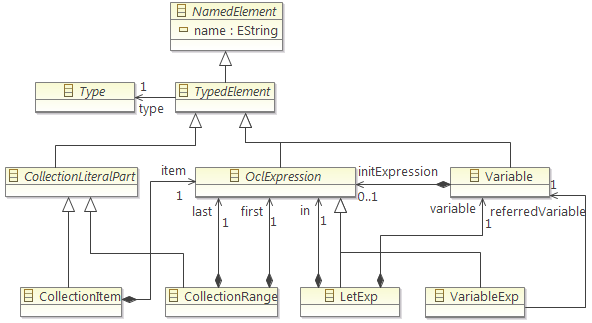
\includegraphics[scale=0.75]{images/RunningaExampleAS.png}
\caption{OCL abstract syntax partial Metamodel}
\label{fig:exampleAS}
\end{figure}

\subsection{Collection literal part}

The parts of a collection literal expression in OCL are provided by \textit{collection literal part}s. Listing~\ref{lst:CollectionLiteralExpExample} is an example of a collection literal expression comprising three comma-separated collection literal parts.

\begin{lstlisting}[label=lst:CollectionLiteralExpExample, language=OCL]
Sequence{1, 1+1, 3..9+1} -- equivalent to Sequence{1,2,3,4,5,6,7,8,9,10}
\end{lstlisting}

To be more specific, a collection literal part could either be a simple element (i.e comprising one expression) of a collection, or a collection range which represents an integer range between two expressions. The rationale of choosing this particular OCL construct is two fold: it will be used to show why the OMG specification is faulty, thus, motivate the need for a better DSL to declare CS2AS bridges (Section~\ref{sec:semi-formal-solution}); and we can show the essence of the CS2AS mappings description (Subsection~\ref{subsec:mappings}). Figure~\ref{fig:CollectionLiteralPartCS} shows the CS definitions related to a collection literal expression.

\begin{figure}[htbp]
\centering
\begin{subfigure}{0.5\textwidth}
  \centering
\begin{lstlisting}[language=Xtext]
CollectionLiteralPartCS:
   ExpCS | CollectionRangeCS

CollectionRangeCS:
   ExpCS '..' ExpCS
\end{lstlisting} 
%  \caption{CollectionLiteralPartCS grammar }
%  \label{fig:CollectionLiteralPartCS:a}
\end{subfigure}%
\begin{subfigure}{0.5\textwidth}
  \centering
  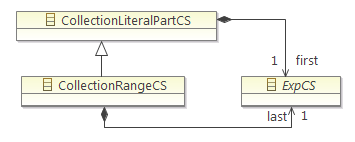
\includegraphics[scale=0.75]{images/CollectionLiteralPartCS.png}
%  \caption{CollectionLiteralPartCS metamodel }
%  \label{fig:CollectionLiteralPartCS:b}
\end{subfigure}
\caption{CollectionLiteralPartCS Grammar and partial CS Metamodel}
\label{fig:CollectionLiteralPartCS}
\end{figure}


\subsection{Let expression}

A \textit{let expression} is used in OCL in order to declare a variable to be used inside another OCL expression. The following listing shows an example of the notation:

\begin{lstlisting}[label=lst:letExpExample, language=OCL]
let var : String = 'something' in var.oclIsTypeOf(String)
\end{lstlisting}

This expression is interesting because it's related to one of the main activities of the CS2AS DSL: name resolution. Whilst a let expression declares a new variable, the \emph{'in'} expression contains a variable expression referring to that variable (note the reference from VariableExp to Variable in the AS excerpt depicted by Figure~\ref{fig:exampleAS}). This activity of creating  references between elements of the AS based on a name lookup is called name resolution (Subsection~\ref{subsec:nameReso}). Figure~\ref{fig:LetExpCS} shows the CS definitions related to a let expression.

\begin{figure}[htbp]
\centering
\begin{subfigure}{0.5\textwidth}
  \centering
  \begin{lstlisting}[label=lst:letExpEBNF, language=Xtext]
LetExpCS:
    'let' VariableDeclarationCS 
  	'in' ExpCS
  	
VariableDeclarationCS:
    simpleName (':' TypeCS)?
    ('=' ExpCS)?	
  \end{lstlisting} 
%  \caption{LetExpCS and VariableDeclarationCS grammar excerpts}
%  \label{fig:LetExpCS:a}
\end{subfigure}%
\begin{subfigure}{0.5\textwidth}
  \centering
  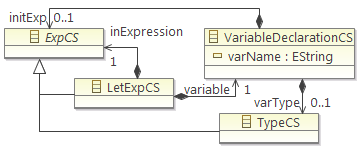
\includegraphics[scale=0.75]{images/LetExpCS.png}
%  \caption{LetExpCS metamodel excerpt}
%  \label{fig:LetExpCS:b}
\end{subfigure}
\caption{LetExpCS Grammar and partial CS Metamodel}
\label{fig:LetExpCS}
\end{figure}

\subsection{Variable expression}

A \textit{variable expression} in OCL references a variable defined elsewhere. The reference may explicitly or implictly refer to the \emph{self} context variable or to an iterator variable, or explicitly to a variable defined in an outer let expression or to a parameter of an operation definition. Discovering and prioritizing the candidate definitions is performed by the name resolution activity. The \emph{varName} provided by a \emph{VariableExpCS} in the concrete syntax is used to look up a \emph{Variable} in the AS. 

Likewise, \textit{variable expression} will be also used to introduce the concern of CS disambiguation in Subection\ref{subsec:disamb}.  Figure~\ref{fig:VariableExpCS} shows the CS definitions related to a variable expression. 

\begin{figure}[htbp]
\centering
\begin{subfigure}{0.5\textwidth}
  \centering
 \begin{lstlisting}[label=lst:VariableExpEBNF, language=Xtext]
 VariableExpCS:
 	simpleName | 'self'
 \end{lstlisting} 
%  \caption{VariableExpCS grammar excerpt}
%  \label{fig:VariableExpCS:a}
\end{subfigure}%
\begin{subfigure}{0.5\textwidth}
  \centering
  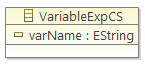
\includegraphics[scale=0.75]{images/VariableExpCS.png}
%  \caption{VariableExp metamodel excerpt}
%  \label{fig:VariableExpCS:b}
\end{subfigure}
\caption{VariableExpCS Grammar and partial CS Metamodel}
\label{fig:VariableExpCS}
\end{figure}



\section{Semi-formal solution: OCL Clause 9.3}
\label{sec:semi-formal-solution}

The OCL specification provides a full attribute grammar in which inherited and synthesized attributes are used to describe how the AS is computed from the CS. Figure~\ref{fig:CollectionLiteralPartOMG} shows an example. The specification uses OCL expressions to express how the different attributes are computed. Attribute grammar are a suitable mechanism to describe a CS2AS bridge; however, we will add some critics about it. 

\begin{figure}[htbp]
\centering
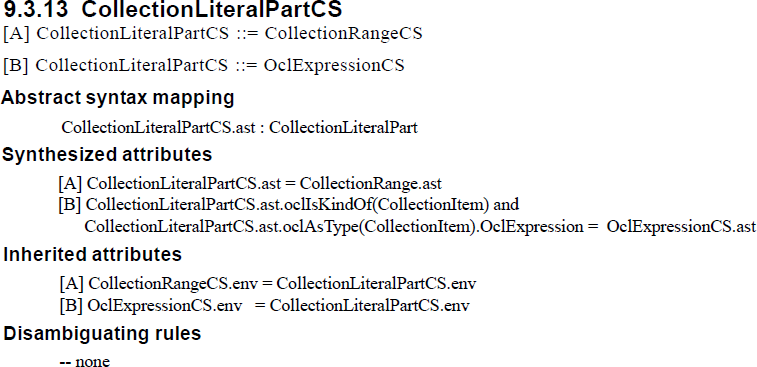
\includegraphics[scale=0.45]{images/CollectionLiteralPartOMG.png}
\caption{OCL specification for CollectionLiteralPartCS to CollectionLiteralPart}
\label{fig:CollectionLiteralPartOMG}
\end{figure}
The first section defines the EBNF production(s). The example merges two alternate productions and so many of the rules have an with \verb$[A]$ or \verb$[B]$ prefix to accommodate the alternative rules.

The AS mapping declares the type of the resulting AS element as the type of a special property of the CS element; \emph{ast}.

The synthesized attributes populate the AS element using a simple assignment for \verb$[A]$. \verb$[B}$ worksaround OCL 2.4's inability to construct objects by imposing constraints on a hypothetical \emph{CollectionItem}.

The inherited attributes contribute to the name resolution by flowing down an Environment hierachy of all available name-element pairs from parent to child nodes using another special CS property; \emph{env}. In this case all names visible in the parent are passed with out modification to the children.

The disambiguating rules provide guidance on the resolution of ambiguities. In this simple example, there is no ambiguity.

\begin{figure}[htbp]
\centering
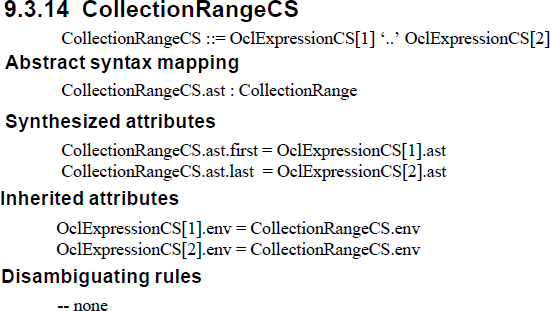
\includegraphics[scale=0.45]{images/CollectionRangeOMG.png}
\caption{OCL specification for CollectionRangeCS to CollectionRange}
\label{fig:CollectionRangeOMG}
\end{figure}
The rules for collection ranges follow a single pattern. There is now just one grammar production whose two OclExpressions are distinguished by \verb$[1]$ and \verb$[2]$ suffixes. The synthesized attributes have two properties to populate.

\textbf{Critique} The presentation comes quite close to specifying what is needed, but uses an intuitive mix of five sub-languages without any tool assistance. In Figure~\ref{fig:CollectionLiteralPartOMG}, the typo whereby the final line of the synthesized attributes uses \emph{CollectionItem::OclExpression} rather than \emph{CollectionItem::item} has gone unreported for over 10 years.

The lack of any underlying models makes it impossible for tool vendors to re-use the rules. Tool vendors must transcribe and risk introducing further errors.

%While attribute grammars are well-suited to describing a CS2AS bridge, they do not lend themselves to standards-compliant tool support. In particular, the declaration of Clause 9.3 from the OCL specification is imprecise, in the sense that it does not conform to any existent language, and there is no tool that vendors can rely on to help to build CS2AS bridges from it, nor to validate the attribute grammars. It would be beneficial to instead be able to use a standard language -- with tool support -- to define CS2AS bridges. Ideally, for OMG languages, it would be beneficial to be able to use a language like OCL to define CS2AS bridges. 

%\textbf{Unchecked CS2AS bridges:} Due to the fact that OCL specification designers came up with their own notation, and there is no tool to check the proposed attribute grammar, we can find errors in Clause 9.3 of the OCL specification. For instance, in Figure~\ref{fig:CollectionLiteralPartOMG} we can see how the second expression that computes the synthesized attributes is incorrect, because, from the OCL AS definition, the property name comprising the OCL expression of a \emph{CollectionItem} is \emph{item}, rather than \emph{OclExpression}

%With these criticisms in mind, in this paper we present a pure OCL-based internal DSL so that existing OCL tools can be used to declare CS2AS bridges so that:

%\begin{itemize}
%\item OMG specification designers can express CS2AS bridges in an OMG language. These bridge definitions will be of higher quality since they can be created and checked using existing OCL tools.
%\item Implementers can benefit from those bridges to build tools supporting OMG specifications comprising textual languages, e.g. by applying MDE techniques (transformations, code generation, etc.).
%\end{itemize}

\section{Modeled Solution: CS2AS internal DSL}
\label{sec:solution}

The critique of the semi-formal exposition highlighted the lack of checkable or re-useable models. In this section we will formalize the semi-formal approach using a DSL to declare the bridge between the CS and the AS of a language. The DSL is  internal\cite{fowler2010dsl} and uses only the facilities proposed for OCL 2.5. The DSL constrains the use of the general purpose OCL language to define  a set of idioms that express CS2AS bridges.

Our rationale for choosing OCL as the host language is as follows:
\begin{itemize}
\item OMG specifications have a problem with bridging the CS to AS gap, so we would like an OMG-based solution.
\item OCL contains a rich expression language which can provide enough flexibility to express non trivial CS2AS bridges in a completely declarative way.
\item Other OMG related languages could be considered (such as one of the QVT languages), however OCL is a well known OMG language and is the basis of many others. A QVT practitioner inherently knows OCL but not vice-versa.
\end{itemize}

Instances of the internal DSL take the form of Complete OCL documents and can be maintained using Complete OCL tools \cite{eclipseOclOnline}. Multiple documents can be used to partition the specification into modules %for topics such as Messages or States and 
to separate the distinct mapping, name-resolution, and disambiguation concerns of the CS2AS bridge.

\subsection{Shadow Object Construction}
\label{subsec:ShadowExp}

The internal DSL uses the proposed\footnote{Shadow object construction was called as type construction in the Aachen report \cite{brucker2013aachenReport}} side-effect-free solution to the problem of constructing types in OCL. This avoids the need for the hypothecated objects used by the semi-formal approach. The proposed syntax re-uses the existing syntax for constructing a Tuple by replacing the \emph{Tuple} keyword by the name of the type to be constructed. A \verb$Complex$ number with \verb$x$ and \verb$y$ parts might therefore be constructed as \verb$Complex{x=1.0,y=2.0}$. %The subtleties of ensuring that construction is side-effect-free are not relevant to this paper.

\subsection{CS2AS mappings}
\label{subsec:mappings}

In this subsection we will explain the main CS2AS mappings description language. We start by introducing an instance of the language so that the reader can have an indication of the DSL used to describe the bridge. Listings ~\ref{lst:exampleCS2ASdescA} and ~\ref{lst:exampleCS2ASdescB} correspond to the CS2AS descriptions of the OCL constructs introduced in the running example (Section~\ref{sec:example}).

\begin{lstlisting}[caption=CS2AS description for a collection literal part, label=lst:exampleCS2ASdescA, language=OCL]
context CollectionLiteralPartCS	
def : ast() : ocl::CollectionLiteralPart = 
  ocl::CollectionItem {
        item = first.ast(),	
        type = first.ast().type
       }
  
context CollectionRangeCS	
def : ast() : ocl::CollectionRange = 
  ocl::CollectionRange {
        first = first.ast(),
        last = last.ast(),
        type = first.ast().type.commonType(last.ast().type)
       }
\end{lstlisting}

The mapping is performed by invoking the \emph{ast()} operation on a CS element. Polymorphic dispatch ensures that the CS element-specific operation is used unlike the \emph{ast} property of the semi-formal approach. The `abstract syntax mapping' and `synthesized attributes' of the semi-formal approach are modeled by the the shadow construction of the appropriate AS type and initialization of its properties. (The initialiization includes the \emph{type} property omitted by the OCL specification.)

\begin{lstlisting}[caption=CS2AS description for let and variable expressions, label=lst:exampleCS2ASdescB, language=OCL]
context LetExpCS
def : ast() : ocl::LetExp = 
  ocl::LetExp {
    variable = variable.ast(),
    _'in' = inExpression.ast(),
    type = inExpression.ast().type
}

context VariableDeclarationCS
def : ast() : ocl::Variable = 
  ocl::Variable {
    name = varName,
    initExpression = initExp.ast(),
    type = if varType = null
           then if initExp = null
                then null
                else initExp.ast().type
                endif
           else varType.ast().type
           endif
}

context VariableExpCS
def : ast() : ocl::VariableExp =
  let variable = ast().lookupVariable(varName)
  in ocl::VariableExp {
       name = varName
       referredVariable = variable
       type = if variable = null
              then null
       	      else variable.type
       	      endif
   	}
\end{lstlisting}

%In this Complete OCL document we have declared the CS2AS bridge to define how AS elements are obtained from CS elements. The bridge is expressed by the means of a correspondence between CS types and AS types. This correspondence is given in terms of operation definitions, so that the operation context type -- an element type in the CS -- is the source of the correspondence, and the operation returned type -- an element type in the AS -- is the target of the correspondence. The actual characteristic function of the correspondence will be described by the body of those operations. For instance, taking as reference Listing~\ref{lst:exampleCS2ASdesc}, the \emph{ast} operation at line 2 defines the correspondence between \emph{LetExp} elements and \emph{LetExpCS} elements. The body of that operation, at lines 3-7, describes how \emph{LetExp} elements (AS) are actually computed from \emph{LetExpCS} elements (CS).

%A more detailed explanation of the whole DSL, as well as the rationale about its design decisions, follows. All the listing and line references below correspond to Listing~\ref{lst:exampleCS2ASdesc}:

\textbf{Declarativeness:} An important characteristic of the DSL is that it comprises declarative OCL constraints. The OCL constraints specify only true correspondences between AS and CS after a valid conversion (FIXME ASBH. Be careful I think this is not true with the ShadowExp usages. I'd not include this sentence). Discovery of a suitable order in which to perform CS to AS conversions requires an implementing tool to analyze the OCL constraints and exploit their inter-dependencies. (This was also the unstated policy of the semi-formal approach.)

\textbf{Operations:} The CS2AS bridge is described by the means of operation definitions. The underlying rationale is that those definitions on a potentially complex class hierarchy of the CS can be overridden. Due to this overriding mechanism, we are providing some flexibility to cope with special cases such as those involving language extensions, as they occur in the OCL and QVT specifications. The operation name is not relevant, but we propose the name \emph{"ast"} because it is aligned with the name used in the attribute grammar exposed in the OCL specification.

\textbf{Shadow object construction:} Shadow object constructions express how AS elements are constructed and how their properties are initialized. %This kind of expression allows the specification of which concrete type is used to bridge towards to (it might differ - be a subtype - from the returned type of the \emph{ast} operation), but also to express how all the corresponding properties of the AS element will be computed. Lines 4-6 shows how a \emph{LetExp} is created from a \emph{LetExpCS}, as well as how the \emph{LetExp::variable}, \emph{LetExp::in} and \emph{LetExp::type} properties are computed.

\textbf{Operation Calls:} To compute properties of any AS element we will normally need to access to other AS elements corresponding to the CS ones. Given that we are using \emph{ast} operations to set a correspondence between CS and AS elements, an \emph{ast} operation call expression (OCE) will be used to denote that we want to obtain the AS element corresponding to the CS element source of that OCE. For example, at line 4, in order to initialize the \emph{LetExp::variable} property, we use the \emph{ast} OCE to obtain the \emph{Variable} corresponding to the \emph{VariableDeclarationCS} belonging to the context \emph{LetExpCS} element (via the \emph{LetExpCS::variable} property).

\textbf{Self-contained:} With the goal in mind of using the proposed internal DSL to rewrite part of the OMG specifications, the declaration of the CS2AS bridge for a particular CS element will be complete and self-contained. This means that the computations for all the properties of the corresponding AS element are expressed in the shadow type expression, even though those properties belong to any of the AS element supertypes. Admitting that the creation of more modularized and reusable declarations is convenient when designing CS2AS bridges, Section~\ref{sec:futureWork} will add additional comments to this topic.
NB ASBH. Perhaps, including the comments in the limitations section (6).

\textbf{Reusable computations:} Having OCL as the  host language for our internal DSL, we could factor out and define more complex and reusable expressions in new operation definitions. Those operations could be reused, by just introducing operation call expressions, across the different computations of the AS element properties. At line 31, we can spot an OCE named \emph{commonType}, which is a reusable operation\footnote{The body of the operation is not relevant, hence, not described in this paper} in charge of computing the common supertype between the source of the OCE, and the provided operation call argument.

\textbf{Name resolution:} As a special case of reusable computation, we want to highlight one which links with Subsection~\ref{subsec:nameReso}: name resolution. It's common a situation in which an AS element refers to a different one based a named-based lookup. In our example, at line 11, we have such scenarios, so that in the context of a \emph{VariableExp} element, there will be a lookup activity triggered by the \emph{lookupVariable} OCE, which aim to find a \emph{Variable} to be referred by that \emph{VariableExp}.

\textbf{Disambiguation:} A CS element doesn't necessarily need to be bridged to just one type of AS element. It's a common situation that preliminary ambiguous CS elements are disambiguated to different AS elements. Subsection~\ref{subsec:disamb} will elaborate on this topic. %We can find varied examples in the OCL specification but \emph{CollectionLiteralPartCS} is an easy to understand one. To describe this scenario in our DSL, we will cascade a set of \emph{IfExp} in the body of the \emph{ast} operation: every condition would comprise a disambiguation rule; the \emph{then} and \emph{else} expressions comprise the shadow type expressions denoting the AS element to which the disambiguation would take place. In our running example, lines 23-33 depicts the mentioned scenario and more details about the called \emph{mapsToCollectionItem} operation will be given in Subsection~\ref{subsec:disamb}: disambiguation.

\subsection{Name resolution description}
\label{subsec:nameReso}
In this subsection, we will explain how name resolution is described when defining CS2AS bridges by the means of our OCL-based internal DSL. In a name resolution activity we can typically find two main roles:
\begin{itemize}
\item a producer provides a name-to-element mapping for all possible elements in its producing scope. 
\item a consumer looks up a specific element corresponding to a name in its consuming context
\end{itemize}
In typical programming languages the use of a variable should have a corresponding declaration. The variable declaration is the be the producer of a name-to-variable mapping. The variable usage consumes the variable by referencing its name. Name resolution searches the hierarchy of producing contexts that surround the consuming context to locate a name-element mapping for the required name.

The semi-formal approach adopted by the OCL specification re-uses the containment hierarchy of the CS as the scope hierarchy for its `inherited attributes'. The name-to-element mappings are mainitained in an Environment hierarchy which flows down from the root CS element to all the leaf elements accumulating additional name-to-element mappings and/or nested environments at each intermediate CS element in the CS tree.

In Section \ref{sec:semi-formal-solution} we saw the very simple unmodified flow-down for a CollectionLiteralPart. The equivalent exposition for a LetExp in the OCL specification is complicated by performing the CS2AS mapping of multiple comma-separated let-variables with respect to the CS rather than the AS. We therefore present its logical equivalent.

\begin{lstlisting}[caption=Semi-formal LetExpCS equivalent, label=lst:semi-formal-letexpcs, language=OCL]
LetExpCS ::= ‘let’ VariableDeclarationCS ‘in’ OclExpressionCS

VariableDeclarationCS.env = LetExpCS.env
OclExpressionCS.env = LetExpCS.env.nestedEnvironment().addElement(VariableDeclarationCS.ast)
\end{lstlisting}

The environment of the LetExpCS is passed unchanged to the VariableDeclarationCS so that name resolution within the VariableDeclarationCS initializer sees the same names as the LextExpCS.

The environment for the OclExpressionCS is more interesting. A nested Environment is created containing the name-to-variable mapping for the let-variable. The use of a nested environment ensures that the let-variable name occludes any same-named mapping in the nested environment.

Although the use of the nestedEnvironment() and addElement() appears to be imperative, a declarative interpretation is possible since addElement() returns a copy of its source environment with an additional name-to-element mapping.

Our modeled approach is very similar but re-uses the AS tree rather than the CS tree as the scope hierarchy. This avoids the complications that arise when resolving syntax sugar such as comma-separated let-variables concurrently.

%In the OCL specification, Clause 9, we might find some hints related to the names resolution activity: On one hand, in Clause 9.4, an \emph{Environment} definition is provided, including some operations to deal with this concept of environment (i.e. a list of named elements); on the other hand in Clause 9.3, the attribute grammar makes uses of those definitions so the environments can be modified, propagated and queried in the CS2AS bridge declaration in order to perform the lookup activities. In the OCL attribute grammar we can spot how the consumers and producers of the lookup activity are interfaced: when an \emph{Environment::addElement/s} operation is invoked we are dealing with a producer, whilst when any form of \emph{lookup} operation is invoked we are dealing with a consumer.

%In essence, an environment comprises a list of named element which can be looked up in other parts of textual  and they can be nested so a child environment can occlude a contribution of a named element with the same name as another contribution done in the parent environment.

%We now explain how name resolution is described in our OCL-based CS2AS DSL. Listing~\ref{lst:exampleNameResodesc} is the name resolution description\footnote{Due to space constraints, just context definitions are included} for our running example; it will be used as a reference when explaining the language design decisions and rationale.

\begin{lstlisting}[caption=Name resolution producers, label=lst:exampleNameResodesc, language=OCL]
context LetExp
def : childEnv(child : OclAny) : env::Environment =
  if child = variable
  then selfEnv()
  else selfEnv().nestedEnv().addElement(variable)
  endif
  
context OclAny
def : _env(child : OclAny) : env::Environment =
  parentEnv()	
\end{lstlisting}

The polymorphic operation \emph{\_env(child)} declares the environment flow down from the LetExp parent to the Variable or OclExpression child using a \emph{child} argument to select which environment is returned.

The default definition of \emph{\_env(child)} flows down the environment to all children. This can be inherited by most AS elements so that only those AS elements such as LetExp that modify the environment need specification.

If each AS element has an \emph{env} property for its Environment, and if the \emph{parentEnv()} helper function just returns \emph{self.env}, the hierarchy of \emph{\_env(child)} operations can be used to flow down the environments from AS root to all AS leaves. In practice this declarative flow down provides large environment hierarchies at each AS leaf where at most one name is actually of interest.

An alternative practical implementation of  the \emph{parentEnv()} helper function and the Environment can exploit the declarative symmetry to search up through the AS hierarchy to ignoring elements that fail to satisfy search criteria such as name or type.

\begin{lstlisting}[caption=Name resolution description for running example, label=lst:exampleNameResodesc, language=OCL]
-- Producers (Environment computation)
context OclAny
def : env() : env::Environment =
  _env(null)
def : _env(child : OclAny) : env::Environment =
  parentEnv()	
def : parentEnv() : env::Environment =
  let parent = oclContainer() 
  in if parent = null 
     then env::Environment { } 
     else parent._env(self) 
     endif
	
context VariableExp
def : _env(child : ocl::OclAny) : env::Environment =
  parentEnv() -- By default, the computed environment is always parentEnv()
                  -- (see line 5) so this declaration might be suppressed

-- Consumers(Lookup computation).
context OclAny 
def : _lookupVariables(env : env::Environment, vName : String) : OrderedSet(Variable) =  	
  let foundVs = env.namedElements->selectByKind(Variable)->select(name=vName) 
  in if foundVs->isEmpty() and not env.parentEnv = null
     then _lookupVariables(env.parentEnv, vName)
     else foundVs 
     endif
     
def : _lookupVariable(vName : String) : Variable =
  let foundVs = _lookupVs(env(), vName)
  in if foundVs->isEmpty()
     then null
     else foundVs->first() 
     endif
     
context VariableExp
def : lookupVariable(varExpCS : oclcs::VariableExpCS) : Variable =
  if varExpCS.varName = null
  then null 
  else _lookupVariable(varExpCS.varName) 
  endif
         
-- Environment related ops
context Environment
def : nestedEnv() : Environment = 
  Environment { 
    parentEnv = self
  }
def : addElements(elements : Collection(ocl::NamedElement)) : Environment =
  Environment {
    parentEnv = parentEnv,
    namedElements = namedElements->includingAll(elements)
  }
def : addElement(element : ocl::NamedElement) : Environment =
  Environment {
    parentEnv = parentEnv,
    namedElements = namedElements->including(element)
  }
\end{lstlisting}

\textbf{Declarativeness}: the definition of consumers and producers of named element lookups is declarative.

\textbf{Bottom up environment computation:} Whereas in the OCL specification the proposed grammar exposes a top down environment computation (in the form of inherited attributes specification), for our internal DSL, the environment computation exposes a bottom up approach. Although declaratively speaking, the approach is irrelevant, in practice the bottom up exposition enables the interpretation or generation of more efficient implementations: in essence, we don't need to carry down the computation of environments along with the entire containment hierarchy (from parents to children); we just need to enable the computation of the environment from the consumer looking for producers above in the containment hierarchy (from children to parents). Lines 2-12 show how an environment is computed by default for an arbitrary element: the bottom line of the algorithm is that, by default, the environment of an element will be the parent (container) element's environment. For a root element (no parent), by default, its environment will comprise an empty list of named elements. 

\textbf{Producer contributions:} In our DSL, a producer will just have to specify an \emph{\_env} operation to declare how it will specifically contribute named elements to the environment. The environment \emph{addElement/s} operations will be used to perform such contribution, being the argument expression the one to express how the contributions are obtained from the producer. Lines 18-23 shows how a \emph{LetExp} producer contributes a \emph{Variable} element to the environment. The \emph{child} parameter of the \emph{\_env} operation is important, since it represents the child element from which a bottom up lookup is being performed. Although not all \emph{\_env} need it, in this case, it is used for \emph{LetExp} at line 20, because we only want to add a \emph{Variable} to the environment in the case that the lookup is performed from the inner \emph{in} expression.

\textbf{Nested environments:} As we can find in many programming languages, a common situation when achieving name resolution is the creation of scopes. Scopes allow name producers to contribute names which might already be defined in outer scopes. In OCL, scopes are represented by the own environments, but we need a way to specify when we want to open a new scope, i.e. create a new nested environment. In our example, \emph{LetExp}  will create a new lookup scope from its parent environment, so that a \emph{nestedEnv} operation call is used at line 21. The \emph{nestEnv} operation is defined at line 50. This producer contribution definition would let variable declarations occlude variables declared by outer \emph{LetExp}, so that the expression in Listing~\ref{lst:nestedEnvExample} would be valid and would return 4 as a result.

\begin{lstlisting}[caption=LetExp variables occlude outer variables, label=lst:nestedEnvExample, language=OCL]
context OclAny
def : a() : Integer =
	let a = 1
	in let a = 2
	   in a + a
\end{lstlisting}
	   
\textbf{Consumer lookups:} \emph{lookup} operations are defined in the context of the consumers for which a lookup needs to be performed (see lines 41-46). Those operations will receive, as an argument, the corresponding CS element from which syntactic information will be retrieved to perform a lookup. In our example, the lookup input corresponds to the String valued \emph{VarExpCS::varName}. The usual lookup inputs will normally be String values, but they can be more complex CS structures such as a PathNameCS (Clause 9.3.7 of \cite{omg2013ocl}) which is used in the OCL specification to perform qualified name lookups. 

The actual lookup is triggered when invoking generic (defined on any OclAny) \emph{\_lookup} operations, which basically consist in computing the environment for the consumer and filtering the resulting list of named elements with the lookup input and the kind of element to look up. In our running example, when looking up \emph{Variable}s, the environment is computed at line 35 and the resulting list of named elements is filtered at line 28.

\textbf{Bottom up lookup computations:} As the reader might have noted, the \emph{\_lookup} operations are designed to be split into two different operations. The rationale is that although we only compute the environment once, an indeterminate number of nested environments might be created. If the looked up element is not found in the list of named elements of the most deep environment, the search must be (transitively) performed in the list of named elements of its parent environment. In our example, the transitive search is exposed at line 30.
\textbf{}

\subsection{Disambiguation}
\label{subsec:disamb}

As we commented in the introduction, CS disambiguation is another important concern which needs to be addressed during the CS2AS bridge. To explain the need of disambiguation rules, let's focus on the following simple OCL expression:

\begin{lstlisting}[language=OCL]
x.y
\end{lstlisting}

In a first glance, \emph{'y'} is a property call expression over an \emph{'x'} variable expression. However, whilst \emph{'y'} is certainly a property call expression , \emph{'x'} doesn't necessarily have to be a variable expression. It actually depends on the context in which that OCL expression is used, because \emph{'x'} could also be another property call expression over the implicit variable \emph{self}, i.e. \emph{self.x.y}. As commented in Section X, The OCL specification doesn't help to clarify this situation, because they provide a wrong (ambiguous) grammar. FIXME ASBH, I'm unsure if the problem with the ambiguous grammar (VariableExpCS[A] and PropertyCallExpCS[B] rules) should be explained here or previously

To sort out this situation, we need to make use of unambiguous CS elements, plus additional disambiguation rules. These rules will specify towards which elements of the AS, an ambiguous CS element will be disambiguated. 

For this particular OCL example, the specification would need to introduce a concept such as \emph{NameExpCS} which simply comprises a name. Figure~\ref{fig:NameExpCS} shows the CS definitions related to an ambiguous name expression. 

\begin{figure}[htbp]
\centering
\begin{subfigure}{0.5\textwidth}
  \centering
 \begin{lstlisting}[label=lst:NameExpEBNF, language=Xtext]
 NameExpCS:
 	simpleName isMarkedPreCS?
 \end{lstlisting} 
%  \caption{VariableExpCS grammar excerpt}
%  \label{fig:VariableExpCS:a}
\end{subfigure}%
\begin{subfigure}{0.5\textwidth}
  \centering
  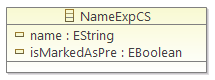
\includegraphics[scale=0.75]{images/NameExpCS.png}
%  \caption{VariableExp metamodel excerpt}
%  \label{fig:VariableExpCS:b}
\end{subfigure}
\caption{NameExpCS Grammar and partial CS Metamodel}
\label{fig:NameExpCS}
\end{figure}

Then, additional disambiguation rules can make use of information from the CS and/or AS, in order to discern which AS element is created from that \emph{NameExpCS} i.e a \emph{VariableExp}, otherwise a \emph{PropertyCallExp}. For instance, Listing~\ref{lst:nameExpDisambiguation} shows the definition for the CS2AS mapping of a \emph{NameExpCS}, in which \emph{isAVariableExp()} operation call is introduced at line 3 and the referenced operation will comprise the disambiguation rule. The reader should not that:

\begin{itemize}
\item VariableExpCS and PropertyCallExpCS metaclasses wouldn't be needed any more. The corresponding VariableExp and PropertyCallExp would be obtained from this ambiguous NameExpCS
\item The ambiguous grammar issue commented before would vanish, since now we have only one grammar rule for NameExpCS. In other words, we have created a CS disambiguation to be resolved in the CS2AS bridge, rather than having an ambiguous grammar.
\end{itemize}

NB ASBH. Problem with this definition, is that we need to define a lookupProperty. It is incorrect/incomplete , and we might to get into a new mess. Omitting the then/else expression might an alternative, but I don't like it....
\begin{lstlisting}[caption=CS2AS description for an ambiguous name expression, label=lst:nameExpDisambiguation, language=OCL]
context NameExpCS
def : ast() : ocl::OclExpression =
  if isAVariableExp() 
  then
    let variable = ast().lookupVariable(self)
    in oclAS::VariableExp {
        name = name,
        referredVariable = variable,
        type = if variable = null
               then null
               else variable.type
               endif
    }
  else 
    let property = ast().lookupProperty(self)
    in oclAS::PropertyCallExp {
        name = name,
        referredProperty = property,
        type = if property = null
               then null
               else property.type
               endif
    }
  endif	
\end{lstlisting}

Disambiguation rules might be simple ones which rely on CS information -- syntactic information --, or more complex ones which also involve AS information -- semantic information --. In the introduced example, we need to rely on AS information to conclude if \emph{'x'} corresponds to a \emph{VariableExp} otherwise a \emph{PropertyCallExp}. Specifically, a lookup using the name comprised by the \emph{NameExpCS} is needed. If we found a \emph{Variable} with that name, we would disambiguate \emph{NameExpCS} towards a \emph{VariableExp}; otherwise towards a \emph{PropertyCallExp}. 

Listing~\ref{lst:nameExpDisambiguationRule} shows the definition of the disambiguation rule for an ambiguous CS element such as \emph{NameExpCS}. The reader should note that we don't consider the case where \emph{'x'} is not neither a variable nor a property of the implicit \emph{self} context variable (an element is not found in the lookup process). We want to provide a declarative and clean CS2AS bridge for the OMG specification. A strict interpretation of the proposed CS2AS bridge for \emph{NameExpCS}, would end up with a \emph{PropertyCallExp} with a null value for the referred property.

\begin{lstlisting}[caption=NameExpCS disambigutation rule, label=lst:nameExpDisambiguationRule, language=OCL]
context NameExpCS
def : isAVariableExp() : Boolean =
	let variable =  ast().lookupVariable(self),
	in variable <> null
\end{lstlisting}

%To conclude the explanation of the proposed OCL based internal DSL, we briefly discuss the CS disambiguation rules which let us produce different AS elements from ambiguous CS element. Disambiguation is a concern different to name resolution, but it is similarly used across the CS2AS mappings definition. The OCL-based descriptions can be defined in their own file and therefore comprise the disambiguation rules for the OMG specification. 

%As we saw in subsection~\ref{subsec:mappings}, in our running example we identified the \emph{mapsToCollectionItem} operation call as the condition required to disambiguate a \emph{CollectionLiteralPartCS} towards either a \emph{CollectionItem} or a \emph{CollectionRange}. Now, Listing~\ref{lst:CS2ASdisambiguation} shows the definition of that \emph{mapsToCollectionItem}, exposing how the rule to disambiguate a \emph{CollectionLiteralPartCS} will depend on the presence (or not) of the \emph{last} expression.
%
%\begin{lstlisting}[caption=CS disambiguation rule of the running example, label=lst:CS2ASdisambiguation, language=OCL]
%context CollectionLiteralPartCS
%def : mapsToCollectionItem() : Boolean =
%	self.last = null
%\end{lstlisting}
%
%As the reader might note, this disambiguation scenario is a trivial one because very little CS information is required to decide if we disambiguate a \emph{CollectionLiteralPartCS} towards either a \emph{CollectionItem} or a \emph{CollectionRange}. Potentially, a more elaborated grammar definition would allow us to prevent any need of a disambiguation rule in this case. However:
%
%\begin{itemize}
%\item The grammar excerpt corresponding to the running example is the one proposed by the specification. Our goal is to provide a flexible DSL that lets us tackle any CS2AS bridging scenario in which we might encounter big CS2AS gaps in favour of more concise grammars (which comprise more ambiguous CS elements when compared with more elaborated grammars).
%\item We can also find more complex disambiguation scenarios in which not only CS (syntactic) information is required, but also AS (semantic) information is needed to disambiguate an ambiguous CS element in a given context. A typical scenario in OCL is when lookups of AS named elements are needed to know if a simple name preceding a \emph{'.'} corresponds to either a variable (hence, VariableExp is the disambiguation result) or to a property of the implicit self variable (hence, PropertyCallExp is the disambiguation result). We can find other related examples in \cite{willink2010oclXtext}.
%\end{itemize}

\section{Related work}
\label{sec:relatedWork}

In this section we will briefly discuss how the proposed OCL-based CS2AS bridge relates to previous work. To the best of our knowledge there does not exist a DSL approach based on OMG specifications to describe bridges between CS and AS. The Complete OCL document based approach was introduced in \cite{sanchez2014enhancingXtext} and this paper aims to explain the whole approach (i.e. the internal DSL).

We can find languages conceived to sort out the CS2AS bridges in other contexts, i.e in the context of some specific tools. %Although our OCL-based internal DSL is appropriate to be used in OMG specifications, we admit that some related works create more convenient constructs for instance, when defining names resolution, or when dealing with reusable bridges defined on abstract classes in the corresponding CS/AS classes hierarchy. 
We highlight two of them:

\textbf{NaBL \cite{konat2013decNameRes} \& Stratego \cite{visser2004stratego}:} These are two separate languages for different purposes used by the Spoofax language workbench \cite{spoofaxOnline}. The former is used to declare name resolution and the latter to declare syntax rewrites (tree based structure transformations). As a main difference with respect to our approach, these languages are completely unrelated: whereas the former is integrated during the parsing activities in order to resolve cross-references when producing the CS tree, the latter is a general purpose program transformation language further used to obtain the potentially different AS tree. In our approach, we integrate the name resolution language into a further CS2AS activity, provided that the parsing activity produces a first CS tree. The reason for not integrating name resolution during the parsing activity is that for the OCL language, we will be interested in looking up AS elements for which we don't have the corresponding input file, just a model conforming to the AS syntax (e.g the OCL Standard library model).

\textbf{Gra2Mol \cite{canovas2012gra2mol}:}  Gra2Mol is an approach that is closer in objective to the approach presented in this paper. It is a domain specific transformation language conceived to define those bridges, and as our approach does, the name resolution activity is also declared as part of the transformation language. However, whilst their name resolution relies on explicitly specifying a direct search (thus, the name consumer needs to know where the name producer is located in the syntax tree), our approach for specifying name resolution is more declarative based on a independent declaration of name producers and consumer (thus, the name consumer doesn't need to know where the producer is located in the syntax tree). Another difference is that whilst we use OCL as the expression language to express the bridges, they define a structure-shy\footnote{Xpath is an example of this kind of languages} query language instead. They claim that the usage of their query language is more compact and less verbose when compared to using OCL expressions. However, that kind of languages are not suitable from the point of view of OMG specifications. Besides, we can add that structure-shy languages are more error prone or sensitive to changes in the involved metamodels (metamodel evolution): when having a static typed language such OCL, supporting tools can better assist in a metamodel evolution scenario.

\section{Limitations and shortcomings}
\label{sec:limitations}

From the point of view of the OMG specification, we do not identify limitations of the proposed internal DSL. Having OCL as the host language is an ideal solution for OMG specifications, because the instances of the DSL can be directly ported to those specifications in order to precisely define the corresponding CS2AS bridges. Likewise, the flexibility and modularity that Complete OCL documents provide has promise in addressing very large CS2AS gap scenarios.

On the other hand, from the final user point of view, i.e the user of the DSL, and specially when comparing with related work, we perceive that having an external DSL fully designed to deal with concepts related to name resolution (e.g. NaBL) or disambiguation may be more convenient. We discuss this further in the next section when talking about future work.

Another shortcoming to mention is that the DSL is based on the concept of shadow type expression, which is not part of the last version of the OCL specification (2.4), though it is planned to be included in the next OCL version (2.5) \cite{brucker2013aachenReport}\footnote{It's cited in the report as type construction expression, Section 3.1}. The number of OCL tools which can currently be used to validate the CS2AS bridges is limited (we are using Eclipse OCL\cite{eclipseOclOnline} which supports some future OCL 2.5 features).

\section{Ongoing and future work}
\label{sec:futureWork}

Apart from using this OCL-based internal DSL to define CS2AS bridges, we are also producing the Java based source code responsible for obtaining AS models from CS ones. This ongoing work follows  the line drawn in the introduction which highlights that the CS2AS internal DSL can be exploited by tool implementers. Although in this paper we are unable to go into further detail, we can point the reader out to some JUnit test cases\footnote{http://git.eclipse.org/c/mmt/org.eclipse.qvtd.git/tree/tests/org.eclipse.qvtd.cs2as.
compiler.tests/src/org/eclipse/qvtd/cs2as/compiler/tests/OCL2QVTiTestCases.java} working on small examples, which demonstrate that the instances of the CS2AS internal DSL can be transformed to executable code and perform the CS2AS gap resolution of a language.

In terms of future work, we highlight the following.

\begin{itemize}
\item \textbf{Definition of CS2AS bridges for OCL and QVT.} We will apply the proposed OCL-based internal DSL to provide complete CS2AS bridge descriptions for the whole OCL and the three QVT languages. We expect these CS2AS bridges will be included as part of the future OCL and QVT specifications. Likewise, since we can generate executable code, we plan  -- in the context of Eclipse OCL and QVTd projects -- to replace some hand-written source code by auto-generated source code produced from the same CS2AS bridge descriptions.

\item \textbf{Creation of an external DSL.} By bringing together the good aspects of other related languages such as NaBL or Gra2Mol, we want to create an external DSL with a higher level of abstraction than the one presented here, to ease even more the creation of those bridges. This external DSL would embed the OCL expressions language, and the supporting tooling would include a code generator to modularly produce the instances of the internal DSL presented in this paper.

\item \textbf{Integration with existing language workbenches.} As added value of the DSL and to provide more proofs about how tool vendors may benefit from it (not covered in this paper), we want to exploit the proposed DSL in the context of a modern language workbench called Xtext.

%\item \textbf{OMG specification generation.} Due to the fact  CS2AS bridges 

\end{itemize}

\section{Conclusions}
\label{sec:conclusions}

OMG specifications, comprising textual languages, can be improved by providing  DSLs to express how the CS can be bridged to the AS. Although some specifications attempt to define those bridges, for instance, by the means of an attribute grammar formalism, these CS2AS bridge definitions contain errors or are incomplete, introducing the motivation to improve the existing means to define them. We have proposed an OCL-based internal DSL for that purpose, and explained, along with a running example, the different aspects of the language. Given the flexibility, modularity and reuse facilities the OCL host language provides, we have showed how CS2AS mappings, name resolution and CS disambiguation can be described in a declarative, modular and sound way. To conclude, we have mentioned all the potential work that this CS2AS internal DSL can provide, and pointed out some publicly available examples in which this CS2AS bridges were exercised, including  ongoing work about the generation of executable source code to perform the CS2AS gap resolution. We claim that those CS2AS bridge descriptions are free of typos, because an existing OCL tool was used to specify them, which will increase the quality of OMG specifications as soon as those descriptions are contributed.

\bibliographystyle{unsrt}
\bibliography{ow2015}

\end{document}